\documentclass[main.tex]{subfiles}

\begin{document}
\chapter{Concept Design}
\chaplabel{conceptDesign}

\section{Platform Selection}
A platform is used as a means to mount the required detection equipment and to act as the foundation for a completely autonomous system.  Design and construction of the platform is not in the scope of the project and so the modification of an existing platform was the preferred approach. The selected platforms included in the decision process were based directly on their availability to the project, whether a commercial product or the loan of equipment. Primary factors that were considered during the selection process were taken from the Project Specifications (see \secref{performance}) and the Project Scope (see \secref{projectScope}). The following list outlines the criterion used during the process and the decision matrix (\figref{platformDecision}). In general, a score of 5 indicated that a requirement had only just been satisfied or that the criterion was only just feasible for that platform, with any difference being representative of a rise or fall in the platforms capability with respect to that requirement. Scores had a lower limit of 1 and an upper limit of 10.
\begin{itemize}
\item Cost: Based on a budget of \$16,500. A platform cost nearing \$5,000 indicated that the requirement had been met. A score of 10 indicates platform supplied in-kind and 1 indicates financially infeasible.
\item Implementation of Auto-Control: How involved the process of implementing the direct hardware required for remote operation would be. A low score indicates a difficult process with many sub-systems, whereas a high score indicates little to no work necessary. Requirement was met if implementation of hardware was a feasible task.
\item Control/Manoeuvrability: How appropriate the platform was expected to be regarding manoeuvrability assuming auto-control was implemented successfully. This included speed, acceleration, turn radius, and stopping distance.
\item Implementation of detection equipment: Ease of installation of detection equipment and expected effectiveness of the platform and sensor combination from a landmine detection point of view.
\item Payload: Platform's ability to support the required 100 kg payload.
\item Terrain Traversing: How capable the platform is at traversing the required terrain. This includes dry and loose sand or gravel with minimum obstacles and a 15 degree gradient.
\item Portability: Level of portability. A higher score indicates simpler transport with less disassembly required. The requirement had been satisfied if transport was possible in the back of a ute or trailer.
\item Operation Time: {\color{red}{need something here, i dont think theres anything in requirements for it yet}}
\item Navigation: How direct and efficient the path of the platform for mine-detecting purposes was expected to be. This involves aspects such as duration and tightness of turns and mine avoidance techniques.
\end{itemize}

\begin{figure}[ht]
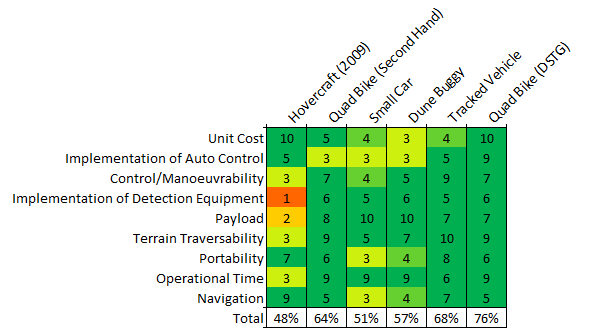
\includegraphics{4-ConceptDesign/platformDecision.png}
\centering
\caption{Platform Decision Matrix} \figlabel{platformDecision}
\end{figure}

\Figref{platformDecision} summarises each of the available platforms which are detailed further in following subsections. If a criterion is met with a score of 5 or higher it is coloured green, otherwise the colour transitions to red - a score of 1. It was evident that the hovercraft did not meet majority of the requirements to be the supporting platform. Commercial quad bikes, small cars, or dune buggies could have been used with some modifications to the structure, however a tracked vehicle or the quad bike offered by DSTG were clearly the two best options.

The DSTG quad bike was selected over a tracked vehicle for a number of reasons. These included direct availability, financial restrictions, and the completed state of auto control hardware already on the quad bike.

\subsection{Hovercraft}
Access was made available to an existing hovercraft from a 2009 Adelaide University Honours Project. Analysis of the technical report \parencite{hovercraft2009} and practical and theoretical evaluations showed that the lift fan was able to support a payload of up to 22 kg and the thrust fans were only just capable of moving the craft on a flat, smooth surface. For complete automation only actuators for the lift motor would be required as remote operation for the thrust system had already been implemented. The stopping distance is lacking due to the time required to rotate fans for reverse thrust. The hovercraft has an advantage over other platforms through its ability to pass directly over a mine without detonation occurring, however, this 'sliding' advantage introduces new problems when developing a path tracking algorithm due to the advanced dynamics of the platform. The purchasing of a recreational hovercraft more suited to the requirements would not have been financially feasible. Through verbal discussion with DSTG, it was revealed that vibrations produced through the lift and thrust systems on hovercraft platforms were detrimental to the effectiveness of the sensor equipment. Thus, the DSTG has advised against the use of a hovercraft as the platform for mine-detecting purposes.
\begin{figure}[ht]
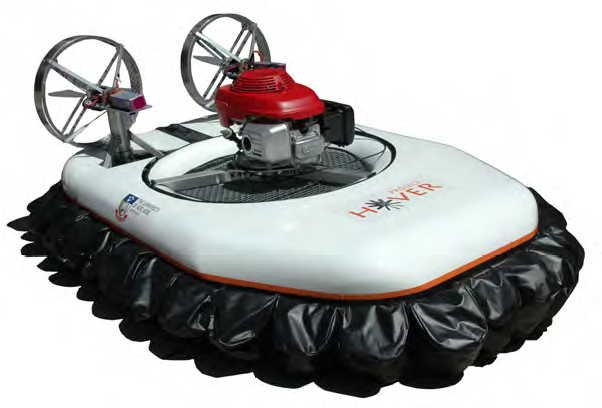
\includegraphics[width=0.4\textwidth]{4-ConceptDesign/HovercraftPic.png}
\centering
\caption[2009 Adelaide University Honours Project Hovercraft]{2009 Adelaide University Honours Project Hovercraft \parencite{hovercraft2009}} \figlabel{hovercraftPic}
\end{figure}

\subsection{Quad Bike}
Quad bikes are designed as all terrain vehicles and are capable of traversing even the most demanding terrains. Utility quad bikes are intended to carry large loads as well as a human operator and so load limits are frequently larger than 100 kg. Due to the nature of the platform and through visual inspection, mounting points for sensor brackets and electronic systems are located in various positions.  Environmental conditions are of little concern to this platform which will be encountered and traversed with ease for ranges of over 100 km. Turning radius for quad bikes are typically in the range of 3-4 metres.
The DSTG have offered the use of one of their autonomous quad bikes to be used as the platform. The DSTG quad bike is a Honda TRX450r and has a weight load capacity of 110 kg. The quad bike has been previously fitted with remote control capabilities and is in good working condition, however \textcite{scheiner2011} recommended that the brake actuator be replaced as well as some electronics. As the platform already has remote control capabilities, transport becomes a much easier task especially with a trailer or ute with a ramp.
\begin{figure}[ht]
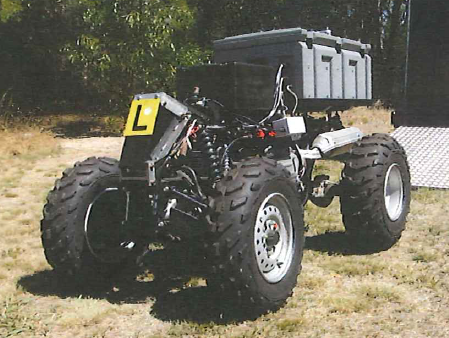
\includegraphics[width=0.4\textwidth]{4-ConceptDesign/2011quadbike.PNG}
\centering
\caption[DSTG Autonomous Quad Bike]{DSTG Autonomous Quad Bike \parencite{scheiner2011}} \figlabel{2011quadbike}
\end{figure}

\subsection{Small Car ?}
turn radius' of around 30 feet.

\subsection{Dune Buggy ?}

\subsection{Tracked Vehicle}

\section{Navigation}
The navigation system is responsible for communicating to the quad bike two primary functions, how to follow a low curvature path and how to turn a specified angle. Platform navigation will be primarily handled via waypoints. After a region is selected by a user it is broken down into a series of waypoints which, once connected, will form a path for the quad bike. In the alternate use case, the navigation system will operate based directly on waypoints created from a user defined path.

\Textcite{snider2009} provides an empirical comparison of path following algorithms and is shown in \figref{trackingComparison}. Tracking Methods are ordered by implementation difficulty from least difficult to most difficult.\\
\textcolor{red}{This figure 4.4 one is an issue since the writing is smaller than our font. Either find a new comparison or redo it with larger text or better colours... :/}
\begin{figure}[ht]
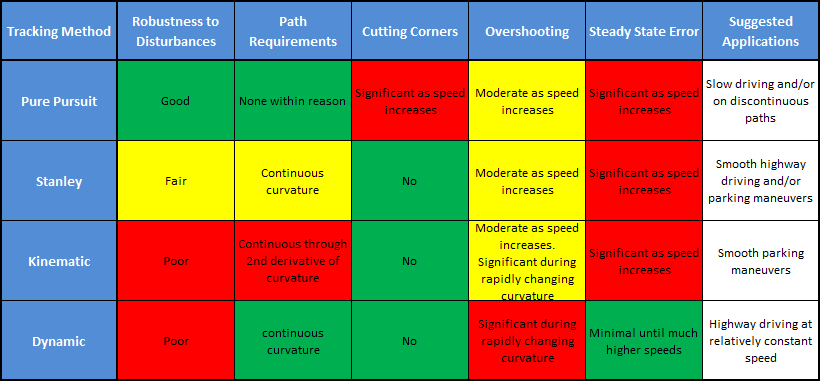
\includegraphics[width = \textwidth]{4-ConceptDesign/pathTrackingSummary.png}
\centering
\caption{Empirical Comparison of Path Tracking Algorithms \parencite{snider2009}} \figlabel{trackingComparison}
\end{figure}


\section{Signal Processing}

\section{Electronics}

\section{Sensor Mount}

\end{document}